\documentclass{ximera}

\input{../preamble.tex}

\title[Dig-In:]{Quadric surfaces}

\begin{document}
\begin{abstract}
  We will get to know some basic quadric surfaces.
\end{abstract}
\maketitle

As we have seen, if we look at the set of points that satisfy an
equation
\[
F(x,y,z)=0
\]
where $F:\R^3\to\R$, we obtain a surface in $\R^3$. A basic class of
surfaces are the \textit{quadric surfaces}.

\begin{definition}
A \dfn{quadric surface} in $\R^3$ is a surface of the form
\[
Ax^2 + By^2 + Cz^2 + Dxy + Exz+ Fyz + Gx + Hy + I z + J = 0
\]
where $A$, $B$, $C$, $D$, $E$, $F$, $G$, $H$, $I$, and $J$ are
constants and at least one of $A$, $B$, $C$, $D$, $E$, or $F$ are
nonzero.
\end{definition}

\begin{warning}
  Do not confuse a \textit{quadric} with a quadratic, or quartic, as
  these are different beasts entirely.
\end{warning}

We will be interested in a special class of quadric surfaces, those
that arise naturally when computing the Taylor polynomial of a surface
$z=F(x,y)$ at a point $\vec{c}$ where:
\[
F^{(1,0)}(\vec{c}) = 0 = F^{(0,1)}(\vec{c})
\]
In this case, the quadric is of the form:
\begin{align*}
  z = &F^{(2,0)}(\vec{c})(x-c_1)^2 \\
  &+ F^{(0,2)}(\vec{c})(y-c_2)^2 \\
  &+ F^{(1,1)}(\vec{c}) (x-c_1)(y-c_2)\\
  &+ F(\vec{c})
\end{align*}
Why are we doing this?
\begin{quote}
  \textbf{Understanding quadric surfaces will help us find extrema of
    surfaces.}
\end{quote}

In what follows, we will study each shape by considering various
\textit{sections} of the surface.

\begin{definition}
  The \dfn{section} of a surface is the intersections of
  a surface with a plane.
\end{definition}

Let's get to it.


\section{Elliptic paraboloids}

An elliptic paraboloid is a surface with graph:
\begin{image}
  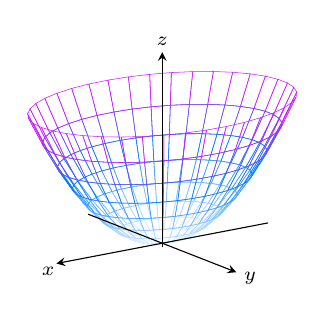
\begin{tikzpicture}
    \begin{axis}%
      [width=175pt,tick label style={font=\scriptsize},axis on top,
	axis lines=center,
	view={145}{20},
	name=myplot,
	xtick=\empty,
	ytick=\empty,
	ztick=\empty,
	ymin=-2.5,ymax=2.5,
	xmin=-3.5,xmax=3.5,
	zmin=-.1, zmax=5.5,
	every axis x label/.style={at={(axis cs:\pgfkeysvalueof{/pgfplots/xmax},0,0)},xshift=-3pt,yshift=-3pt},
	xlabel={\scriptsize $x$},
	every axis y label/.style={at={(axis cs:0,\pgfkeysvalueof{/pgfplots/ymax},0)},xshift=5pt,yshift=-2pt},
	ylabel={\scriptsize $y$},
	every axis z label/.style={at={(axis cs:0,0,\pgfkeysvalueof{/pgfplots/zmax})},xshift=0pt,yshift=4pt},
	zlabel={\scriptsize $z$},
        colormap/cool
      ]
      
      \addplot3[domain=0:360,y domain=0:2,color=black!40,mesh,samples=40,samples y=10,very thin,z buffer=sort] ({2*cos(x)*y},{sin(x)*y},{y^2});
    \end{axis}
  \end{tikzpicture}
\end{image}
and equation:
\[
z=\pm\frac{x^2}{a^2}\pm\frac{y^2}{b^2}
\]
To understand this surface better consider the trace when:
\begin{itemize}
  \item $x=d$, in this case we now have $z = \pm\frac{d^2}{a^2} \pm
    \frac{y^2}{b^2}$, a parabola.
  \item $y=d$, in this case we now have $z = \pm\frac{x^2}{a^2} \pm
    \frac{d^2}{b^2}$, a parabola.
  \item $z=d$, in thisi case we now have $d = \pm\frac{x^2}{a^2} \pm
    \frac{y^2}{b^2}$, an ellipse.
\end{itemize}
\begin{image}
  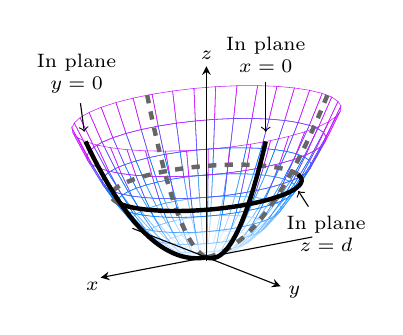
\begin{tikzpicture}
    \begin{axis}%
      [width=175pt,tick label style={font=\scriptsize},axis on top,
	axis lines=center,
        clip=false,
	view={145}{20},
	name=myplot,
	xtick=\empty,
	ytick=\empty,
	ztick=\empty,
	ymin=-2.5,ymax=2.5,
	xmin=-3.5,xmax=3.5,
	zmin=-.1, zmax=5.5,
	every axis x label/.style={at={(axis cs:\pgfkeysvalueof{/pgfplots/xmax},0,0)},xshift=-3pt,yshift=-3pt},
	xlabel={\scriptsize $x$},
	every axis y label/.style={at={(axis cs:0,\pgfkeysvalueof{/pgfplots/ymax},0)},xshift=5pt,yshift=-2pt},
	ylabel={\scriptsize $y$},
	every axis z label/.style={at={(axis cs:0,0,\pgfkeysvalueof{/pgfplots/zmax})},xshift=0pt,yshift=4pt},
	zlabel={\scriptsize $z$},colormap/cool
      ]
      
      \addplot3[domain=0:360,y domain=0:2,mesh,samples=40,samples y=10,very thin,z buffer=sort] ({2*cos(x)*y},{sin(x)*y},{y^2});
      
      \addplot3[domain=170:360,dashed,ultra thick,smooth,samples y=0,black!60,%surf,%fill=white,
        samples=30,] ({2*cos(x)*sqrt(2)},{sin(x)*sqrt(2)},{2});

      \addplot3[domain=-2:0,dashed,ultra thick,smooth,samples y=0,black!60,%surf,%fill=white,
        samples=30,] ({2*x},{0},{x^2});

      \addplot3[domain=-2:0,dashed,ultra thick,smooth,samples y=0,black!60,%surf,%fill=white,
        samples=30,] ({0},{x},{x^2});
      
      \addplot3[domain=0:170,ultra thick,smooth,samples y=0,black,%surf,%fill=white,
        samples=30,] ({2*cos(x)*sqrt(2)},{sin(x)*sqrt(2)},{2});
      
      \addplot3[domain=0:2,ultra thick,smooth,samples y=0,black,%surf,%fill=white,
        samples=30,] ({2*x},{0},{x^2});

      \addplot3[domain=0:2,ultra thick,smooth,samples y=0,black,%surf,%fill=white,
          samples=30,] ({0},{x},{x^2});
      
        \draw (axis cs:4.3,0,6) node[align=center] (A1) {\scriptsize In plane\\[-4pt] \scriptsize $y=0$};
        \draw (axis cs:4,0,4) node (A2) {};
        \draw [->](A1)--(A2);
        
        \draw (axis cs:0,2,6.5) node[align=center] (B1) {\scriptsize In plane\\[-4pt] \scriptsize $x=0$};
        \draw (axis cs:0,2,4) node (B2) {};
        \draw [->](B1)--(B2);

        \draw (axis cs:-2,2,1) node[align=center] (C1) {\scriptsize In plane\\[-4pt] \scriptsize $z=d$};
        \draw (axis cs:-2.83,0,2) node [below] (C2) {};
        \draw [->](C1)--(C2);
        %\foreach \z in {-6.28,-4.71,-1.57,1.57,6.28}
        %{\addplot3[domain=-2:2,,thick,smooth,samples y=0,{\colortwo},%surf,%fill=white,
        %samples=30,] ({sin(deg(\z))},{x},{\z});
        %}
    \end{axis}
  \end{tikzpicture}
\end{image}
\[
\begin{array}{cc}
\textbf{Plane} & \textbf{Section} \\ \hline
x=d  & \text{Parabola} \\
y=d  & \text{Parabola}\\
z=d  & \text{Ellipse}
\end{array}
\]




\section{Hyperbolic paraboloids}

A hyperbolic paraboloid is a surface with graph:
\begin{image}
  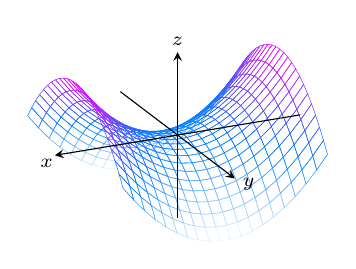
\begin{tikzpicture}[>=stealth]
    \begin{axis}%
      [width=175pt,tick label style={font=\scriptsize},axis on top,
	axis lines=center,
	view={155}{30},
	name=myplot,
	xtick=\empty,
	ytick=\empty,
	ztick=\empty,
	ymin=-1.2,ymax=1.2,
	xmin=-1.2,xmax=1.2,
	zmin=-1.2, zmax=1.2,
	every axis x label/.style={at={(axis cs:\pgfkeysvalueof{/pgfplots/xmax},0,0)},xshift=-3pt,yshift=-3pt},
	xlabel={\scriptsize $x$},
	every axis y label/.style={at={(axis cs:0,\pgfkeysvalueof{/pgfplots/ymax},0)},xshift=5pt,yshift=-2pt},
	ylabel={\scriptsize $y$},
	every axis z label/.style={at={(axis cs:0,0,\pgfkeysvalueof{/pgfplots/zmax})},xshift=0pt,yshift=4pt},
	zlabel={\scriptsize $z$},
        colormap/cool
      ]

      \addplot3[domain=-1:1,smooth,y domain=-1:1,mesh,samples=20,samples y=25,very thin,z buffer=sort] ({x},{y},{x^2-y^2});
    \end{axis}
  \end{tikzpicture}
\end{image}
and equation:
\[
z=\pm\frac{x^2}{a^2}\mp\frac{y^2}{b^2}
\]
To understand this surface better consider the trace when:
\begin{itemize}
  \item $x=d$, in this case we now have $z = \pm\frac{d^2}{a^2} \mp
    \frac{y^2}{b^2}$, a parabola.
  \item $y=d$, in this case we now have $z = \pm\frac{x^2}{a^2} \mp
    \frac{d^2}{b^2}$, a parabola that opens the \textit{opposite}
    direction as the previous one.
  \item $z=d$, in thisi case we now have $d = \pm\frac{x^2}{a^2} \mp
    \frac{y^2}{b^2}$, a hyperbola.
\end{itemize}
\begin{image}
  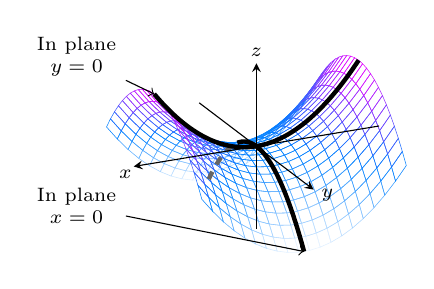
\begin{tikzpicture}
    \begin{axis}%
      [width=175pt,tick label style={font=\scriptsize},axis on top,
	axis lines=center,
	view={155}{30},
	name=myplot,
	xtick=\empty,
	ytick=\empty,
	ztick=\empty,
	ymin=-1.2,ymax=1.2,
	xmin=-1.2,xmax=1.2,
	zmin=-1.2, zmax=1.2,
	every axis x label/.style={at={(axis cs:\pgfkeysvalueof{/pgfplots/xmax},0,0)},xshift=-3pt,yshift=-3pt},
	xlabel={\scriptsize $x$},
	every axis y label/.style={at={(axis cs:0,\pgfkeysvalueof{/pgfplots/ymax},0)},xshift=5pt,yshift=-2pt},
	ylabel={\scriptsize $y$},
	every axis z label/.style={at={(axis cs:0,0,\pgfkeysvalueof{/pgfplots/zmax})},xshift=0pt,yshift=4pt},
	zlabel={\scriptsize $z$},colormap/cool
      ]
      
      \addplot3[domain=-1:1,smooth,y domain=-1:1,mesh,samples=20,samples y=25,very thin,z buffer=sort] ({x},{y},{x^2-y^2});

      \addplot3[domain=-1:-.4,dashed,ultra thick,smooth,samples y=0,black!60,%surf,%fill=white,
        samples=30,] ({0},{x},{-x^2});
      
      \addplot3[domain=-1:1,ultra thick,smooth,samples y=0,black,%surf,%fill=white,
        samples=30,] ({x},{0},{x^2});
      
      \addplot3[domain=-.4:1,ultra thick,smooth,samples y=0,black,%surf,%fill=white,
        samples=30,] ({0},{x},{-x^2});
      
      
      \draw (axis cs:1.,0,1) node (A2) {};
      \draw (axis cs:0,1,-1) node (B2) {};
      %\draw (axis cs:0,1.5,0.3) node (C2) {};
      
    \end{axis}
    
    \draw (0,3) node [align=center](A1) {\scriptsize In plane\\[-4pt] \scriptsize $y=0$};
    \draw (0,1.1) node [align=center](B1) {\scriptsize In plane\\[-4pt] \scriptsize $x=0$};
    %
    \draw [->](A1)--(A2.center);
    \draw [->](B1)--(B2.center);
    %\draw [->](C1)--(C2.center);
  \end{tikzpicture}
\end{image}
We'll give an addtional graph to show the hyperbolas:
\begin{image}
  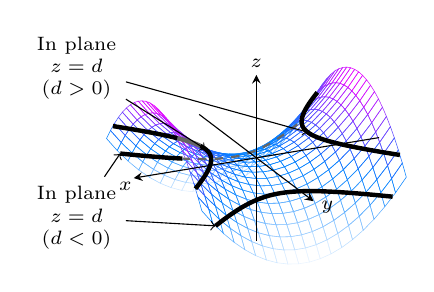
\begin{tikzpicture}
\begin{axis}%
  [width=175pt,tick label style={font=\scriptsize},axis on top,
    axis lines=center,
    view={155}{30},
    name=myplot,
    xtick=\empty,
    ytick=\empty,
    ztick=\empty,
    ymin=-1.2,ymax=1.2,
    xmin=-1.2,xmax=1.2,
    zmin=-1.2, zmax=1.2,
    every axis x label/.style={at={(axis cs:\pgfkeysvalueof{/pgfplots/xmax},0,0)},xshift=-3pt,yshift=-3pt},
    xlabel={\scriptsize $x$},
    every axis y label/.style={at={(axis cs:0,\pgfkeysvalueof{/pgfplots/ymax},0)},xshift=5pt,yshift=-2pt},
    ylabel={\scriptsize $y$},
    every axis z label/.style={at={(axis cs:0,0,\pgfkeysvalueof{/pgfplots/zmax})},xshift=0pt,yshift=4pt},
    zlabel={\scriptsize $z$},
    colormap/cool
  ]

  \addplot3[domain=-1:1,y domain=-1:1,mesh,samples=20,samples y=25,very thin,z buffer=sort] ({x},{y},{x^2-y^2});
  
  \addplot3[domain=-10:60,ultra thick,smooth,samples y=0,black,%surf,%fill=white,
    samples=30,] ({.5*sec(x)},{.5*tan(x)},{.25});
  \addplot3[domain=-35:-10,ultra thick,smooth,samples y=0,black!60,%surf,%fill=white,
    samples=30,] ({.5*sec(x)},{.5*tan(x)},{.25});
  \addplot3[domain=-60:-35,ultra thick,smooth,samples y=0,black,%surf,%fill=white,
    samples=30,] ({.5*sec(x)},{.5*tan(x)},{.25});
  
  \addplot3[domain=-60:60,ultra thick,smooth,samples y=0,black,%surf,%fill=white,
    samples=30,] ({-.5*sec(x)},{.5*tan(x)},{.25});
  
  
  \addplot3[domain=-60:60,ultra thick,smooth,samples y=0,black,%surf,%fill=white,
    samples=30,] ({.5*tan(x)},{.5*sec(x)},{-.25});
  \addplot3[domain=40:60,ultra thick,smooth,samples y=0,black,%surf,%fill=white,
    samples=30,] ({.5*tan(x)},{-.5*sec(x)},{-.25});
  \addplot3[domain=-60:40,dashed,thick,smooth,samples y=0,black!60,%surf,%fill=white,
    samples=30,] ({.5*tan(x)},{-.5*sec(x)},{-.25});

  \draw (axis cs:.5,0,.25) node (A2) {};
  \draw (axis cs:-.5,0,.25) node (A3) {};
  \draw (axis cs:.866,1,-.25) node (B2) {};
  \draw (axis cs:.866,-1,-.25) node (B3) {};
  %\draw (axis cs:0,1.5,0.3) node (C2) {};
\end{axis}
\draw (0,3) node [align=center](A1) {\scriptsize In plane\\[-4pt] \scriptsize $z=d$\\[-4pt] \scriptsize $(d>0)$};
\draw (0,1.1) node [align=center](B1) {\scriptsize In plane\\[-4pt] \scriptsize $z=d$\\[-4pt] \scriptsize $(d<0)$};
%\draw (4.6,2) node [align=center](C1) {\scriptsize in plane\\[-4pt] \scriptsize $z=0$};

\draw [->](A1)--(A2.center);
\draw [->](A1)--(A3.center);
\draw [->](B1)--(B2.center);
\draw [->](B1)--(B3.center);
%\draw [->](C1)--(C2.center);
  \end{tikzpicture}
\end{image}
\[
\begin{array}{cc}
\textbf{Plane}  & \textbf{Section} \\ \hline
x=d & \text{Parabola}\\
y=d & \text{Parabola}\\
z=d & \text{Hyperbola}
\end{array}
\]

\section{Identifying quadric surfaces}

In this course, we will be looking at quadric surfaces of the form: 
\begin{align*}
  z = &F^{(2,0)}(\vec{c})(x-c_1)^2\\
  &+ F^{(0,2)}(\vec{c})(y-c_2)^2 \\
  &+ F^{(1,1)}(\vec{c}) (x-c_1)(y-c_2)\\
  &+ F(\vec{c}).
\end{align*}
and trying to identify them as either a elliptic paraboloid, or a
hyperboloic paraboloid. In what follows, let
\[
\sign(x) =
\begin{cases}
  1  &\text{if $x>0$,}\\
  -1 &\text{if $x<0$,}\\
  0  &\text{if $x=0$.}
\end{cases}
\]
This will aid in our analysis of the quadric surfaces.

\subsection{The pure partials have opposite signs}
If
\[
\sign(F^{(2,0)}(\vec{c})) = -\sign(F^{(0,2)}(\vec{c})),
\]
then we can examine the following sections:
\[
y= c_2 \quad\text{and}\quad x = c_1
\]
If $y=c_2$ then the surface
\begin{align*}
  z = &F^{(2,0)}(\vec{c})(x-c_1)^2\\
  &+ F^{(0,2)}(\vec{c})(y-c_2)^2 \\
  &+ F^{(1,1)}(\vec{c}) (x-c_1)(y-c_2)\\
  &+ F(\vec{c}).
\end{align*}
becomes
\[
z = F^{(2,0)}(\vec{c})(x-c_1)^2 + F(\vec{c}),
\]
and this is a parabola that opens in the $z$ direction of the sign of
$F^{(2,0)}(\vec{c})$.

If $x=c_1$ then the suface becomes
\[
z = F^{(0,2)}(\vec{c})(y-c_2)^2 + F(\vec{c}),
\]
and this is a parabola that opens in the $z$ direction of the sign of
$F^{(0,2)}(\vec{c})$. Since 
\[
\sign(F^{(2,0)}(\vec{c})) = -\sign(F^{(0,2)}(\vec{c})),
\]
we see that when the pure partials have opposite signs, then the
quadric surface is a hyperbolic paraboloid.

\subsection{The pure partials have the same sign}
If 
\[
\sign(F^{(2,0)}(\vec{c})) = \sign(F^{(0,2)}(\vec{c})),
\]
then we start by examining the section
\[
y= c_2
\]
If $y=c_2$ then the surface
\begin{align*}
  z = &F^{(2,0)}(\vec{c})(x-c_1)^2\\
  &+ F^{(0,2)}(\vec{c})(y-c_2)^2 \\
  &+ F^{(1,1)}(\vec{c}) (x-c_1)(y-c_2)\\
  &+ F(\vec{c}).
\end{align*}
becomes
\[
z = F^{(2,0)}(\vec{c})(x-c_1)^2 + F(\vec{c}).
\]
and this is a parabola that opens in the $z$ direction of the sign of
$F^{(2,0)}(\vec{c})$.

When can we find another parabola on this surface that opens in the
opposite direction? Well, let's examine the section
\[
y -c_2 = K (x-c_1).
\]
Substituting this into the surface above, we find
\begin{align*}
  z = &F^{(2,0)}(\vec{c})(x-c_1)^2\\
  &+ K^2 F^{(0,2)}(\vec{c})(x-c_1)^2\\
  &+ K F^{(1,1)}(\vec{c}) (x-c_1)^2 \\
  &+ F(\vec{c}).
\end{align*}
Factoring and rearranging, we find 
\[
z = (x-c_1)^2 \left(
K^2 F^{(0,2)}(\vec{c})(x-c_1)^2 + K F^{(1,1)}(\vec{c}) + F^{(2,0)}(\vec{c})
\right)+ F(\vec{c}).
\]
  and this is a parabola that opens in the $z$ direction of the sign of
$F^{(2,0)}(\vec{c})$. Since 
\[
\sign(F^{(2,0)}(\vec{c})) = -\sign(F^{(0,2)}(\vec{c})),
\]
we see that when the pure partials have opposite signs, then the
quadric surface is a hyperbolic paraboloid.


If
\[
F^{(1,1)}(\vec{c}) =0
\]
then we only need to look at the signs of the second derivatives to
identify the surface. Let
\[
\sign(x) =
\begin{cases}
  1  &\text{if $x>0$,}\\
  -1 &\text{if $x<0$,}\\
  0  &\text{if $x=0$.}
\end{cases}
\]
Now if,
\[
\sign(F^{(2,0)}(\vec{c})) = \sign(F^{(0,2)}(\vec{c}))
\]
our surface is an elliptic paraboloid. On the otherhand if
\[
\sign(F^{(2,0)}(\vec{c})) = -\sign(F^{(0,2)}(\vec{c})),
\]
then our surface is a hyperbolic paraboloid.

\subsection{The mixed derivative is nonzero}


\end{document}

